\documentclass[11pt,final]{article}

\usepackage{multicol}
\usepackage{import}
\usepackage{scn}
\usepackage{microtype}
\usepackage{graphics}
\usepackage[utf8]{inputenc}
\usepackage[left=2cm,right=2cm,top=2cm,bottom=2cm]{geometry}
\usepackage{xcolor}
\usepackage{caption}
\usepackage{float}
\usepackage{enumitem}
\usepackage[russian]{babel}

\setcounter{page}{180}
\renewcommand{\thepage}{\textbf{\arabic{page}}}
\setlength{\intextsep}{-3pt}

\begin{document}
    \begin{multicols}{2}
    
        \noindent\textbf{\textit{abstract non-atomic sc-agent of knowledge extraction from technical documentation}}
        
        {\fontsize{3.4mm}{0}\begin{scnrelfromset}{decomposition of abstract sc-agent:}
            \scnitem{abstract sc-agent of document}
            \textit{ \hspace{2em} preparation}
            \scnitem{abstract sc-agent of standard description}
            \scnitem{abstract sc-agent of ontology description}
            \scnitem{abstract sc-agent of LLM communication}
            \scnitem{abstract sc-agent of LLM responce}
            \textit{ \hspace{2em} parsing}
        \end{scnrelfromset}}
            \vspace{1em}
        \noindent\footnotesize{Figure 2. Decomposition of the abstract non-atomic sc-agent of automated knowledge extraction}

            \vspace{2em}
            
        The sc-agent of document preparation is responsible
        for the preliminary preparation of the document and
        determining the type of standard to which it belongs. The
        document is converted into text form. This process may
        be accompanied by the use of image analysis tools (if
        images are present in the document).

        The sc-agent of standard description is capable of returning a description of the standard to which the document in question was defined. It conveys information about the specific organization of text in documents of a particular standard.

        The sc-agent of ontology description agent is capable of returning a description of the ontology of the subject area (for example, “probabilistic technological production processes”): a set of concepts, their description and a description of the connections between them.

        The sc-agent of LLM communication is responsible for generating a prompt from information collected from previous agents and sending it as a request to the LLM. After sending, the agent expects to receive a response. The agent is not tied to a specific implementation or location of a large language model.

        The sc-agent of LLM response parsing is the key element responsible for checking the correctness of the response received from the large language model (LLM). This agent checks the LLM response for compliance with the data format and consistency with the domain ontology. Its functionality is necessary to account for possible situations of "hallucination" or errors that may occur in the operation of the knowledge extractor-LLM. If the answer is successfully verified, the extracted information can be used to populate the knowledge base. Given the complex nature of the task that this agent needs to solve it may operate also using an LLM.\\

        \begin{center}
            V. An example of extracting information from\\documentation using LLM
        \end{center}

        An example of the information extraction approach can be demonstrated using the project documentation for the PLCnext testbed [22] (Fig. 3, 4, 5).

        \columnbreak

        The documentation contains extensive text on software settings for working with the stand (Fig. 6). Using the described prompt engineering, you can use LLM (ChatGPT 3.5 [17]) to structured knowledge extraction for each configuration step in JSON format, where each instruction step is correctly separated into a separate element (Fig. 7 and 8).

            \vspace{1em}
        {\centering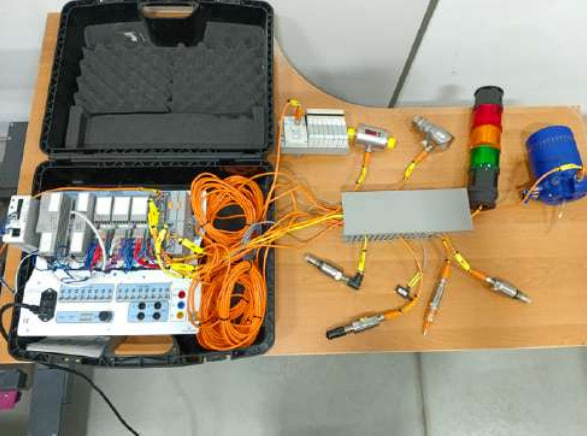
\includegraphics[width=0.5\textwidth]{1_mat.jpg}}
        \begin{center}
            Figure 3. General view of the stand
        \end{center}
            \vspace{1.5em}
        {\centering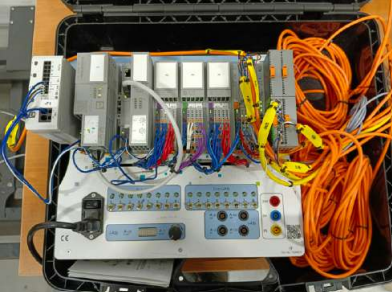
\includegraphics[width=0.5\textwidth]{2_mat.jpg}}
        \begin{center}
            Figure 3. General view of the stand
        \end{center}

            \vspace{0.2em}

        \begin{center}
            VI. Conclusion
        \end{center}
        This paper proposes an approach to solving an important practical problem - automated knowledge extraction
        for constructing enterprise knowledge bases, based on the
        application of an agent-based approach within the framework of OSTIS Technology and the use of large language
        models. The logic of operation of the corresponding
        component of the OSTIS Ecosystem is presented, which
        allows you to systematize and retrieve information from
        various data sources. The described approach can be
        applied not only in the field of enterprises, but also
    \end{multicols}
    
    \newpage
    
    \begin{multicols}{2}
        \begin{figure}[H]
            \centering
            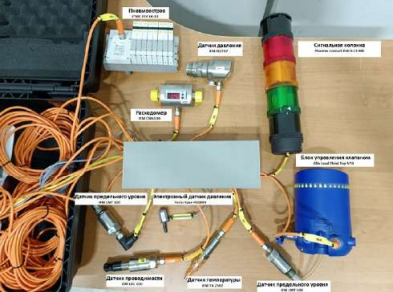
\includegraphics[width=1.0135\linewidth]{3_mat.jpg}
            \label{fig:enter-label}
            {\scriptsize Figure 7. Structured Information Retrieval}
        \end{figure}

        \vspace{1em}

        \begin{figure}[H]
            \centering
            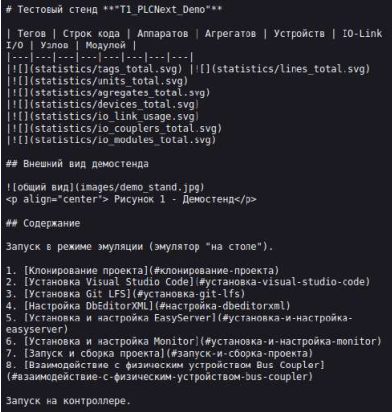
\includegraphics[width=1.0135\linewidth]{4_mat.jpg}
            \label{fig:enter-label}
            {\scriptsize Figure 7. Structured Information Retrieval}
        \end{figure}

        \vspace{1em}

        {\noindent in other subject areas where work with standardized documentation is required as a source for populating knowledge bases.}

        \vspace{-0.3em}
    
        \begin{center}
            References
        \end{center}
        
        \vspace{-3.4em}
        
        \renewcommand{\refname}{}
        \scriptsize\begin{thebibliography}{3} 
            \setlength{\parskip}{-3.5pt}
            \bibitem{1} V. Golenkov, Ed., Tehnologija kompleksnoj podderzhki zhiznennogo cikla semanticheski sovmestimyh intellektual’nyh komp’juternyh sistem novogo pokolenija [Technology of complex life cycle support of semantically compatible intelligent computer systems of new generation]. Bestprint, 2023.
            \bibitem{2} C. D. Manning, H.Schütze Foundations of statistical natural language processing, 1999, MIT press.
            \bibitem{3} V. Taberko, D. Ivaniuk, V. Smorodin, V. Prokhorenko Adaptive Control System for Technological Process within OSTIS Ecosystem, Otkrytye semanticheskie tekhnologii proektirovaniya intellektual’nykh system [Open semantic technologies for intelligent systems], 2023, pp. 291-298.
        \end{thebibliography}

        \columnbreak
        
        \begin{figure}[H]
            \centering
            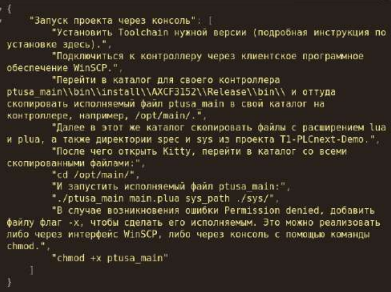
\includegraphics[width=1.0135\linewidth]{5_mat.jpg}
            \label{fig:enter-label}
            {\scriptsize Figure 7. Structured Information Retrieval}
        \end{figure}

            \vspace{1.5em}

        \begin{figure}[H]
            \centering
            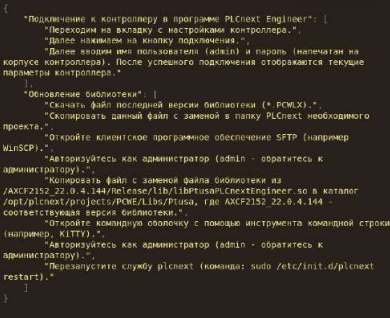
\includegraphics[width=1.0135\linewidth]{6_mat.jpg}
            \label{fig:enter-label}
            {\scriptsize Figure 8. Structured Information Retrieval}
        \end{figure}

            \vspace{-2em}

        \begin{thebibliography}{7} \setcounter{enumiv}{3}
        \setlength{\parskip}{-3.5pt} 
            \scriptsize\bibitem{} V. Taberko, D. Ivaniuk, N. Zotov, M. Orlov, O. Pupena, N. Lutska Principles Of Building A System For Automating The Activities Of A Process Engineer Based On An Ontological Approach Within The Framework Of The Industry 4.0 Concept, System [Open semantic technologies for intelligent systems], 2021, pp. 209-218.
            \scriptsize\bibitem{} “ISA5.1 Standard,” https://www.isa.org/standards-andpublications/isa-standards/isa standards-committees/isa5-1/, (accessed 2024, Jan)
            \scriptsize\bibitem{}  “ISA-88 standard,” Available at: https://www.isa.org/isa88/, (accessed 2024, Jan).
            \scriptsize\bibitem{}   “ISA-95 standard,” https://www.isa.org/standards-andpublications/isa-standards/isa standards-committees/isa95/, (accessed 2024, Jan)
            \scriptsize\bibitem{}  J. Lee, B. Choi A survey of standardization efforts for serviceoriented architecture, Expert Systems with Applications, 2009, 36(4), pp.7844-7855.
            \scriptsize\bibitem{} M. Salama, S.K. Mostefaoui, A. Nour A survey on IoT interoperability and Principles Of standardisation issues, International Journal of Ad Hoc and Ubiquitous Computing, 13(3), 145-155.
            \scriptsize\bibitem{} V. Taberko, D. Ivaniuk, D. Shunkevich, O. Pupena Principles For Enhancing The Development And Use Of StandardsWithin Industry 4.0, Otkrytye semanticheskie tekhnologii proektirovaniya
        \end{thebibliography}
    \end{multicols}
    
    \newpage

    \begin{multicols}{2}

        \renewcommand{\refname}{}
        {\scriptsize\begin{thebibliography}{12} \setcounter{enumiv}{10}
        \setlength{\parskip}{-3.5pt}

            \item[] intellektual’nykh system [Open semantic technologies for intelligent systems], 2020, pp. 167-174.
            \bibitem{}A. Radford, K.Narasimhan, Improving Language Understanding by Generative Pre-Training, 2018
            \bibitem{} J. Devlin, M. Chang, K. Lee, K. Toutanova, BERT: Pre training of Deep Bidirectional Transformers for Language Understanding, 2019 North American Chapter of the Association for Computational Linguistics.
            \bibitem{} Tom B. Brown, Benjamin Mann, Nick Ryder, Melanie Subbiah, Jared Kaplan, Prafulla Dhariwal, Arvind Neelakantan, Pranav Shyam, Girish Sastry, Amanda Askell, Sandhini Agarwal, Ariel Herbert-Voss, Gretchen Krueger, Tom Henighan, Rewon Child, Aditya Ramesh, Daniel M. Ziegler, Jeffrey Wu, Clemens Winter, Christopher Hesse, Mark Chen, Eric Sigler, Mateusz Litwin, Scott Gray, Benjamin Chess, Jack Clark, Christopher Berner, Sam McCandlish, Alec Radford, Ilya Sutskever, Dario Amodei Language models are few-shot learners. arXiv preprint arXiv:2005.14165, 2020
            \bibitem{} D. Xu, Wei C., W. Peng, C. Zhang, T. Xu, X. Zhao, X. Wu, Y. Zheng, E. Chen Large Language Models for Generative Information Extraction: A Survey, 2020, arXiv preprint arXiv:2005.14165.
            \bibitem{} A. Zagorskiy Integration Of Third-Party Functional Services On A Unified Semantic Basis, Otkrytye semanticheskie tekhnologii proektirovaniya intellektual’nykh system [Open semantic technologies for intelligent systems], 2023, pp. 207-212.
            \bibitem{} A. Cherkas, A. Kupo Ostis Technology Integration With ThirdParty NLP Services, Otkrytye semanticheskie tekhnologii proektirovaniya intellektual’nykh system [Open semantic technologies for intelligent systems], 2023, pp. 207-212.
            \bibitem{} “Introducing ChatGPT”, Available at: https://openai.com/blog/chatgpt, (accessed 2023, January).
            \bibitem{} P.Kohli, R.Gupta, S.Saxena, Robustness Challenges in Language Models: A Survey. arXiv preprint arXiv:2103.01021, 2021
            \bibitem{} J. Dodge, S.Gururangan, D.Card, R.Schwartz, N. A.Smith, S. R.Bowman Fine-tuning language models from human preferences. arXiv preprint arXiv:1909.08593, 2020
            \bibitem{} A. Holtzman, J. Buys, J. Du, M. Forbes, Y.Choi, The curious case of neural text degeneration. arXiv preprint arXiv:1904.09751, 2020
            \bibitem{} Y. Liu, M.Ott, N. Goyal, J. Du, M.Joshi, D.Chen, V. Stoyanov, Roberta: A robustly optimized BERT pretraining approach, arXiv preprint arXiv:1907.11692, 2019
            \bibitem{} “T1-PLCnext-Demo”, Available at: https://github.com/savushkinr-d/T1-PLCnext-Demo, (accessed 2023, January).
        \end{thebibliography}}
        
        \columnbreak
            
        \begin{minipage}{0.4\textwidth}
            \begin{center}
                {\normalsize{\textbf{NLP ПОДХОД К ПОСТРОЕНИЮ БАЗЫ ЗНАНИЙ ПРЕДПРИЯТИЯ С ИСПОЛЬЗОВАНИЕМ БОЛЬШИХ ЯЗЫКОВЫХ МОДЕЛЕЙ }}}
            \end{center}
            \begin{center}
                {\small\textbf{Таберко В. В., Иванюк Д. С.,
                Смородин В. С., Прохоренко В. А.}}
            \end{center}

        Предложен подход к автоматизированному формированию базы знаний о предприятии на основании анализа существующей технической документации с применением больших языковых моделей. Данный подход позволяет обеспечить возможность интеграции предлагаемого решения с другими разработками, программными средствами предприятия для обеспечения построения интеллектуальных систем автоматизированного управления, рекомендательных систем и систем поддержки принятия решений, систем информационного обеспечения персонала предприятия.

        \begin{flushright}
            Received 13.03.2024
        \end{flushright}

        \end{minipage}
    \end{multicols}
\end{document}